\documentclass[dvips, lscape]{foils}
%\documentclass[dvips, french]{slides}
\textwidth 18.5cm
\textheight 25cm 
\topmargin -1cm 
\oddsidemargin  -1cm 
\evensidemargin  -1cm

% Maths
\usepackage{amsfonts, amsmath, amssymb}

\newcommand{\coefbin}[2]{\left( 
    \begin{array}{c} #1 \\ #2 \end{array} 
  \right)}
\newcommand{\bbullet}{\bullet\bullet}
\newcommand{\bbbullet}{\bbullet\bullet}
\newcommand{\bbbbullet}{\bbbullet\bullet}
\newcommand{\Bcal}{\mathcal{B}}
\newcommand{\Ccal}{\mathcal{C}}
\newcommand{\Dcal}{\mathcal{D}}
\newcommand{\Ecal}{\mathcal{E}}
\newcommand{\Mcal}{\mathcal{M}}
\newcommand{\Ncal}{\mathcal{N}}
\newcommand{\Pcal}{\mathcal{P}}
\newcommand{\Qcal}{\mathcal{Q}}
\newcommand{\Lcal}{\mathcal{L}}
\newcommand{\Tcal}{\mathcal{T}}
\newcommand{\Ucal}{\mathcal{U}}
\newcommand{\Xcal}{\mathcal{X}}
\newcommand{\Zcal}{\mathcal{Z}}
\newcommand{\etabar}{\overline{\eta}}
\newcommand{\pibar}{\overline{\pi}}
\newcommand{\alphabf}{\mbox{\mathversion{bold}{$\alpha$}}}
\newcommand{\betabf}{\mbox{\mathversion{bold}{$\beta$}}}
\newcommand{\gammabf}{\mbox{\mathversion{bold}\newcommand{\psibf}{\mbox{\mathversion{bold}{$\psi$}}}
{$\gamma$}}}
\newcommand{\mubf}{\mbox{\mathversion{bold}{$\mu$}}}
\newcommand{\psibf}{\mbox{\mathversion{bold}{$\psi$}}}
\newcommand{\Sigmabf}{\mbox{\mathversion{bold}{$\Sigma$}}}
\newcommand{\taubf}{\mbox{\mathversion{bold}{$\tau$}}}
\newcommand{\thetabf}{\mbox{\mathversion{bold}{$\theta$}}}
\newcommand{\Abf}{{\bf A}}
\newcommand{\Ebf}{{\bf E}}
\newcommand{\Hbf}{{\bf H}}
\newcommand{\Ibf}{{\bf I}}
\newcommand{\Sbf}{{\bf S}}
\newcommand{\mbf}{{\bf m}}
\newcommand{\ubf}{{\bf u}}
\newcommand{\vbf}{{\bf v}}
\newcommand{\xbf}{{\bf x}}
\newcommand{\Xbf}{{\bf X}}
\newcommand{\Esp}{{\mathbb E}}
\newcommand{\Corr}{{\mathbb C}\mbox{orr}}
\newcommand{\Var}{{\mathbb V}}
\newcommand{\Ibb}{{\mathbb I}}
\newcommand{\Rbb}{\mathbb{R}}
\newcommand{\Vsf}{\mathsf{V}}

% Couleur et graphiques
\usepackage{color}
\usepackage{graphics}
\usepackage{epsfig} 
\usepackage{pstcol}

% Texte
\usepackage{lscape}
\usepackage{../../../../Latex/fancyheadings, rotating, enumerate}
%\usepackage[french]{babel}
\usepackage[latin1]{inputenc}
%\definecolor{darkgreen}{cmyk}{0.5, 0, 0.5, 0.5}
%\definecolor{green}{cmyk}{0.5, 0, 0.5, 0.5}
\definecolor{orange}{cmyk}{0, 0.6, 0.8, 0}
\definecolor{jaune}{cmyk}{0, 0.5, 0.5, 0}
\newcommand{\textblue}[1]{\textcolor{blue}{#1}}
\newcommand{\textred}[1]{\textcolor{red}{#1}}
\newcommand{\textgreen}[1]{\textcolor{green}{ #1}}
\newcommand{\textlightgreen}[1]{\textcolor{green}{#1}}
%\newcommand{\textgreen}[1]{\textcolor{darkgreen}{#1}}
\newcommand{\textorange}[1]{\textcolor{orange}{#1}}
\newcommand{\textyellow}[1]{\textcolor{yellow}{#1}}
\newcommand{\refer}[2]{{\sl #1}}

% Sections
%\newcommand{\chapter}[1]{\centerline{\LARGE \textblue{#1}}}
% \newcommand{\section}[1]{\centerline{\Large \textblue{#1}}}
% \newcommand{\subsection}[1]{\noindent{\Large \textblue{#1}}}
% \newcommand{\subsubsection}[1]{\noindent{\large \textblue{#1}}}
% \newcommand{\paragraph}[1]{\noindent {\textblue{#1}}}
% Sections
\newcommand{\chapter}[1]{
  \addtocounter{chapter}{1}
  \setcounter{section}{0}
  \setcounter{subsection}{0}
%  {\centerline{\LARGE \textblue{\arabic{chapter} - #1}}}
  {\centerline{\LARGE \textblue{#1}}}
  }
\newcommand{\section}[1]{
  \addtocounter{section}{1}
  \setcounter{subsection}{0}
%  {\centerline{\Large \textblue{\arabic{chapter}.\arabic{section} - #1}}}
  {\centerline{\Large \textblue{#1}}}
  }
\newcommand{\subsection}[1]{
  \addtocounter{subsection}{1}
%  {\noindent{\large \textblue{\arabic{chapter}.\arabic{section}.\arabic{subsection} - #1}}}
  {\noindent{\large \textblue{#1}}}
  }
\newcommand{\paragraph}[1]{\noindent{\textblue{#1}}}

%%%%%%%%%%%%%%%%%%%%%%%%%%%%%%%%%%%%%%%%%%%%%%%%%%%%%%%%%%%%%%%%%%%%%%
%%%%%%%%%%%%%%%%%%%%%%%%%%%%%%%%%%%%%%%%%%%%%%%%%%%%%%%%%%%%%%%%%%%%%%
%%%%%%%%%%%%%%%%%%%%%%%%%%%%%%%%%%%%%%%%%%%%%%%%%%%%%%%%%%%%%%%%%%%%%%
%%%%%%%%%%%%%%%%%%%%%%%%%%%%%%%%%%%%%%%%%%%%%%%%%%%%%%%%%%%%%%%%%%%%%%
\begin{document}
%%%%%%%%%%%%%%%%%%%%%%%%%%%%%%%%%%%%%%%%%%%%%%%%%%%%%%%%%%%%%%%%%%%%%%
%%%%%%%%%%%%%%%%%%%%%%%%%%%%%%%%%%%%%%%%%%%%%%%%%%%%%%%%%%%%%%%%%%%%%%
%%%%%%%%%%%%%%%%%%%%%%%%%%%%%%%%%%%%%%%%%%%%%%%%%%%%%%%%%%%%%%%%%%%%%%
%%%%%%%%%%%%%%%%%%%%%%%%%%%%%%%%%%%%%%%%%%%%%%%%%%%%%%%%%%%%%%%%%%%%%%
\landscape
\newcounter{chapter}
\newcounter{section}
\newcounter{subsection}
\setcounter{chapter}{0}
\headrulewidth 0pt 
\pagestyle{fancy} 
\cfoot{}
\rfoot{\begin{rotate}{90}{
      \hspace{1cm} \tiny S. Robin: A mixture model for random graphs 
      }\end{rotate}}
\rhead{\begin{rotate}{90}{
      \hspace{-.5cm} \tiny \thepage
      }\end{rotate}}

%%%%%%%%%%%%%%%%%%%%%%%%%%%%%%%%%%%%%%%%%%%%%%%%%%%%%%%%%%%%%%%%%%%%%%
%%%%%%%%%%%%%%%%%%%%%%%%%%%%%%%%%%%%%%%%%%%%%%%%%%%%%%%%%%%%%%%%%%%%%%
\begin{center}
  \textblue{\LARGE A mixture model for random graphs} 

   \vspace{1cm}
   {\large J-J Daudin, F. Picard, \underline{S. Robin}} \\
   robin@inapg.inra.fr

   {UMR INA-PG / ENGREF / INRA SSB, Paris} \\
   {Math�matique et Informatique Appliqu�es}
   
\end{center}

\hspace{-1.8cm}
\begin{tabular}{ll}
  \paragraph{Working group:} & E. Birmel�, C. Matias, F. Muri (Evry
   univ.), \\
   & S. Schbath (INRA-MIG)
\end{tabular}

\vspace{1cm}

\subsection{Data = biological network} \\
Protein interaction network, reaction network, enzyme network, {\it etc.}

\subsection{Problem: Find groups of vertices} \\
Groups of proteins, reactions, enzymes according to the connections
between them.

%%%%%%%%%%%%%%%%%%%%%%%%%%%%%%%%%%%%%%%%%%%%%%%%%%%%%%%%%%%%%%%%%%%%%
%%%%%%%%%%%%%%%%%%%%%%%%%%%%%%%%%%%%%%%%%%%%%%%%%%%%%%%%%%%%%%%%%%%%%
\newpage
\chapter{Random graph}
%%%%%%%%%%%%%%%%%%%%%%%%%%%%%%%%%%%%%%%%%%%%%%%%%%%%%%%%%%%%%%%%%%%%%

\paragraph{Notation and definition.} Given a set of $n$ vertices ($i = 1..n$),
$X_{ij}$ indicates the presence/absence of a (non oriented) edge
between vertices $i$ and $j$:
$$
X_{ij} = X_{ji} = \left\{ 
  \begin{array}{rl}
    1 & \mbox{if } i \leftrightarrow j, \\
    0 & \mbox{otherwise}
  \end{array} \right.
\qquad X_{ii} = 0.
$$
The random graph is defined by the join distribution of all the
edges $\{X_{ij}\}_{i, j}$.

\vspace{1cm}
\paragraph{Typical characteristics.} 

\noindent\begin{tabular}{ll}
  Degree (connectivity) of the vertices: & ${K_i = \sum_{j
      \neq i} X_{ij}}$ \\
  \\
  Clustering coefficient: &  ${c = \Pr\{X_{jk} = 1 \;|\;
    X_{ij} = X_{ik} = 1 \}}$ \\
  \\
  Diameter: & Longest path between two vertices.
\end{tabular}

%%%%%%%%%%%%%%%%%%%%%%%%%%%%%%%%%%%%%%%%%%%%%%%%%%%%%%%%%%%%%%%%%%%%%
\newpage
\subsection{Erd�s-R�nyi (ER) model}

\paragraph{Definition.} The $\{X_{ij}\}_{i, j}$ are i.i.d.: 
$$
X_{ij} \sim \Bcal(p).  
$$

\paragraph{Characteristics.}

\noindent\begin{tabular}{ll}
  Degree: & $K_i \sim \Bcal(n-1, p) \approx \Pcal(\lambda)$ \\
  \\
  Clustering coefficient: &  ${c = p}$ \\
\end{tabular}


\vspace{1cm}
\paragraph{Drawback.} The ER fits poorly many real-world networks.
\begin{itemize}
\item Empirical degree distributions are often very different from the
  Poisson distribution because of few vertices having very high
  degrees.
\item Empirical clustering coefficients are generally higher than
  expected under ER.
\end{itemize}

%%%%%%%%%%%%%%%%%%%%%%%%%%%%%%%%%%%%%%%%%%%%%%%%%%%%%%%%%%%%%%%%%%%%%
\newpage
\chapter{Mixture model for the degrees} \label{Sec:PoissonMixture}
%%%%%%%%%%%%%%%%%%%%%%%%%%%%%%%%%%%%%%%%%%%%%%%%%%%%%%%%%%%%%%%%%%%%%

\paragraph{Scale-free distribution.} The most popular alternative to
the Poisson distribution is the Zipf distribution:
$$
\Pr\{K = k\} = c(\rho)k^{-(\rho+1)},
$$
where $\rho > 0$ and $c(\rho)$ is a normalizing constant. (Not
defined for $k = 0$.)

\bigskip\bigskip
\paragraph{Mixture model.} We propose to generalize the ER model
assuming that the vertices belong to $Q$ different groups with
different mean degrees $\lambda_q$. 

We denote $\alpha_q$ the prior probability (proportion) of each group
$$
\alpha_q = \Pr\{i \in q\}, 
\quad 
\sum_q \alpha_q = 1
$$
and $Z_{iq}$ the binary variable indicating if vertex $i$ belongs
to group $q$:
$
Z_{iq} = \Ibb\{i \in q\}.
$

%%%%%%%%%%%%%%%%%%%%%%%%%%%%%%%%%%%%%%%%%%%%%%%%%%%%%%%%%%%%%%%%%%%%%
\newpage
\paragraph{Distribution of the degrees.} $K$ has a mixture
distribution
$$
K \sim \sum_q \alpha_q \Pcal(\lambda_q)
\qquad \Rightarrow \qquad
\Pr \{ K = k \}= \sum_{q=1}^Q \alpha_q \frac{e^{-\lambda_q} \lambda_q^k}{k!}.
$$

%%%%%%%%%%%%%%%%%%%%%%%%%%%%%%%%%%%%%%%%%%%%%%%%%%%%%%%%%%%%%%%%%%%%%
\subsection{Application to {\it E. coli} reaction network}

\begin{itemize}
\item \vspace{-0.5cm} $n = 605$ vertices (reactions) and $1\;782$
  edges. 
\item \vspace{-0.5cm} 2 reactions $i$ and $j$ are connected if the
  product of $i$ is the substrate of $j$ (or conversely).
\item \vspace{-0.5cm} provided by V. Lacroix and M.-F. Sagot (INRIA
H�lix).
\end{itemize}

\paragraph{Parameter estimates.} The BIC criterion select $Q = 3$ groups:
$$
\begin{tabular}{cccc}
  group & 1 & 2 & 3 \\
  \hline
  $\widehat{\alpha}$ (\%) & 8.9 & 19.7 & 71.3 \\
  $\widehat{\lambda}$ & 21.5 & 9.1 & 3.0 \\
\end{tabular}
$$

%%%%%%%%%%%%%%%%%%%%%%%%%%%%%%%%%%%%%%%%%%%%%%%%%%%%%%%%%%%%%%%%%%%%%
\newpage
\paragraph{Distribution fits.} 
$$
\begin{tabular}{cccc}
  Distribution & \begin{tabular}{c}log-log plot \\ / histogram
  \end{tabular} & \multicolumn{2}{c}{P-P plot} \\ 
%  \\
  \hline
  \begin{tabular}{c} Zipf \end{tabular}
  & \begin{tabular}{c} \epsfig{file = ../figures/log_log.eps,
      height=5cm, width = 5cm} \end{tabular}
  & \begin{tabular}{c} \epsfig{file = ../figures/PPplot1.eps,
      height=5cm, width = 5cm} \end{tabular}
  & \begin{tabular}{c} \epsfig{file = ../figures/PPplot6.eps, height=5cm, width =
      5cm} \end{tabular} \\ 
  & & threshold = 1 & threshold = 6 \\
  \hline
%  \\
  \begin{tabular}{c} Poisson \\ mixture \end{tabular}
  & \begin{tabular}{c} 
    %\epsfig{file = ../figures/degre_melange.eps, height=5cm, width=5cm} 
    \epsfig{file = ../figures/ECOli-Poisson-Q3.eps, height=5cm,
    width=5cm, angle=90, bbllx=335, bblly=415, bburx=555, bbury=700, clip=}  
  \end{tabular}
  & \begin{tabular}{c} 
    %\epsfig{file = ../figures/PPplot_melange.eps, height=5cm, width=5cm} 
    \epsfig{file = ../figures/ECOli-Poisson-Q3.eps, height=5cm,
    width=5cm, angle=90, bbllx=65, bblly=80, bburx=285, bbury=360, clip=} 
  \end{tabular} \\
\end{tabular}
$$
%\paragraph{Preliminary conclusions.}
\begin{itemize}
\item \vspace{-0.5cm} The Poisson mixture fits the data well, better
  than the Zipf model.
\item \vspace{-0.5cm} But a model for the degrees is still not a
  random graph model.
\end{itemize}


%%%%%%%%%%%%%%%%%%%%%%%%%%%%%%%%%%%%%%%%%%%%%%%%%%%%%%%%%%%%%%%%%%%%%
%%%%%%%%%%%%%%%%%%%%%%%%%%%%%%%%%%%%%%%%%%%%%%%%%%%%%%%%%%%%%%%%%%%%%
\newpage
\chapter{Erd�s-R�nyi mixture for graph (ERMG)} \label{Sec:ErdosMixture}
%%%%%%%%%%%%%%%%%%%%%%%%%%%%%%%%%%%%%%%%%%%%%%%%%%%%%%%%%%%%%%%%%%%%%

%%%%%%%%%%%%%%%%%%%%%%%%%%%%%%%%%%%%%%%%%%%%%%%%%%%%%%%%%%%%%%%%%%%%%
\subsection{An explicit random graph model} 

\paragraph{Mixture population of vertices.} We still suppose that the
vertices belong to $Q$ groups:
$$
\alpha_q = \Pr\{i \in q\}, 
\qquad
Z_{iq} = \Ibb\{i \in q\}.
$$

\paragraph{Conditional distribution of the edges.}
The edges $\{X_{ij}\}$ are conditionally independent given the group of
the vertices:
$$
X_{ij} \; |\; \{i \in q, j \in \ell \} \sim \Bcal(\pi_{q\ell}).
$$
$\pi_{q\ell} = \pi_{\ell q}$ is the connection probability between
groups $q$ and $\ell$.

A high value of $\pi_{q\ell}$ reveals a preferential connectivity
between groups $q$ and $\ell$. 


%%%%%%%%%%%%%%%%%%%%%%%%%%%%%%%%%%%%%%%%%%%%%%%%%%%%%%%%%%%%%%%%%%%%%
\newpage
\subsection{Examples} 
%%%%%%%%%%%%%%%%%%%%%%%%%%%%%%%%%%%%%%%%%%%%%%%%%%%%%%%%%%%%%%%%%%%%%

%$$
\begin{tabular}{lcccc}
  Description & Network & $Q$ & $\pi$
  & \begin{tabular}{c} Clustering \\ coefficient \end{tabular}\\
  \hline
  \begin{tabular}{p{2cm}} `Random' \end{tabular}
  & \begin{tabular}{c}\epsfig{file = ../figures/FigNetworks-Erdos.eps, height=1.7cm,
      width=2.5cm, clip=, bbllx=120, bblly=260, bburx=530,
      bbury=570}  \end{tabular}
  & 1
  &  $p$ & $p$ \\
  \hline
  \begin{tabular}{p{2cm}} Independent model (product connectivity) \end{tabular}
  & \begin{tabular}{c}\epsfig{file = ../figures/FigNetworks-Indep.eps,
      height=2cm, width=4cm, clip=, bbllx=120, bblly=260, bburx=530,
      bbury=570}  \end{tabular}
  & 2
  & $\left( \begin{array}{cc} a^2 &ab\\ ab&b^2\\ \end{array}
  \right)$
  & $\displaystyle{\frac{(a^2+b^2)^2}{(a+b)^2}}$ \\
  \hline
  \begin{tabular}{p{2cm}} Stars \end{tabular}
  & \begin{tabular}{c}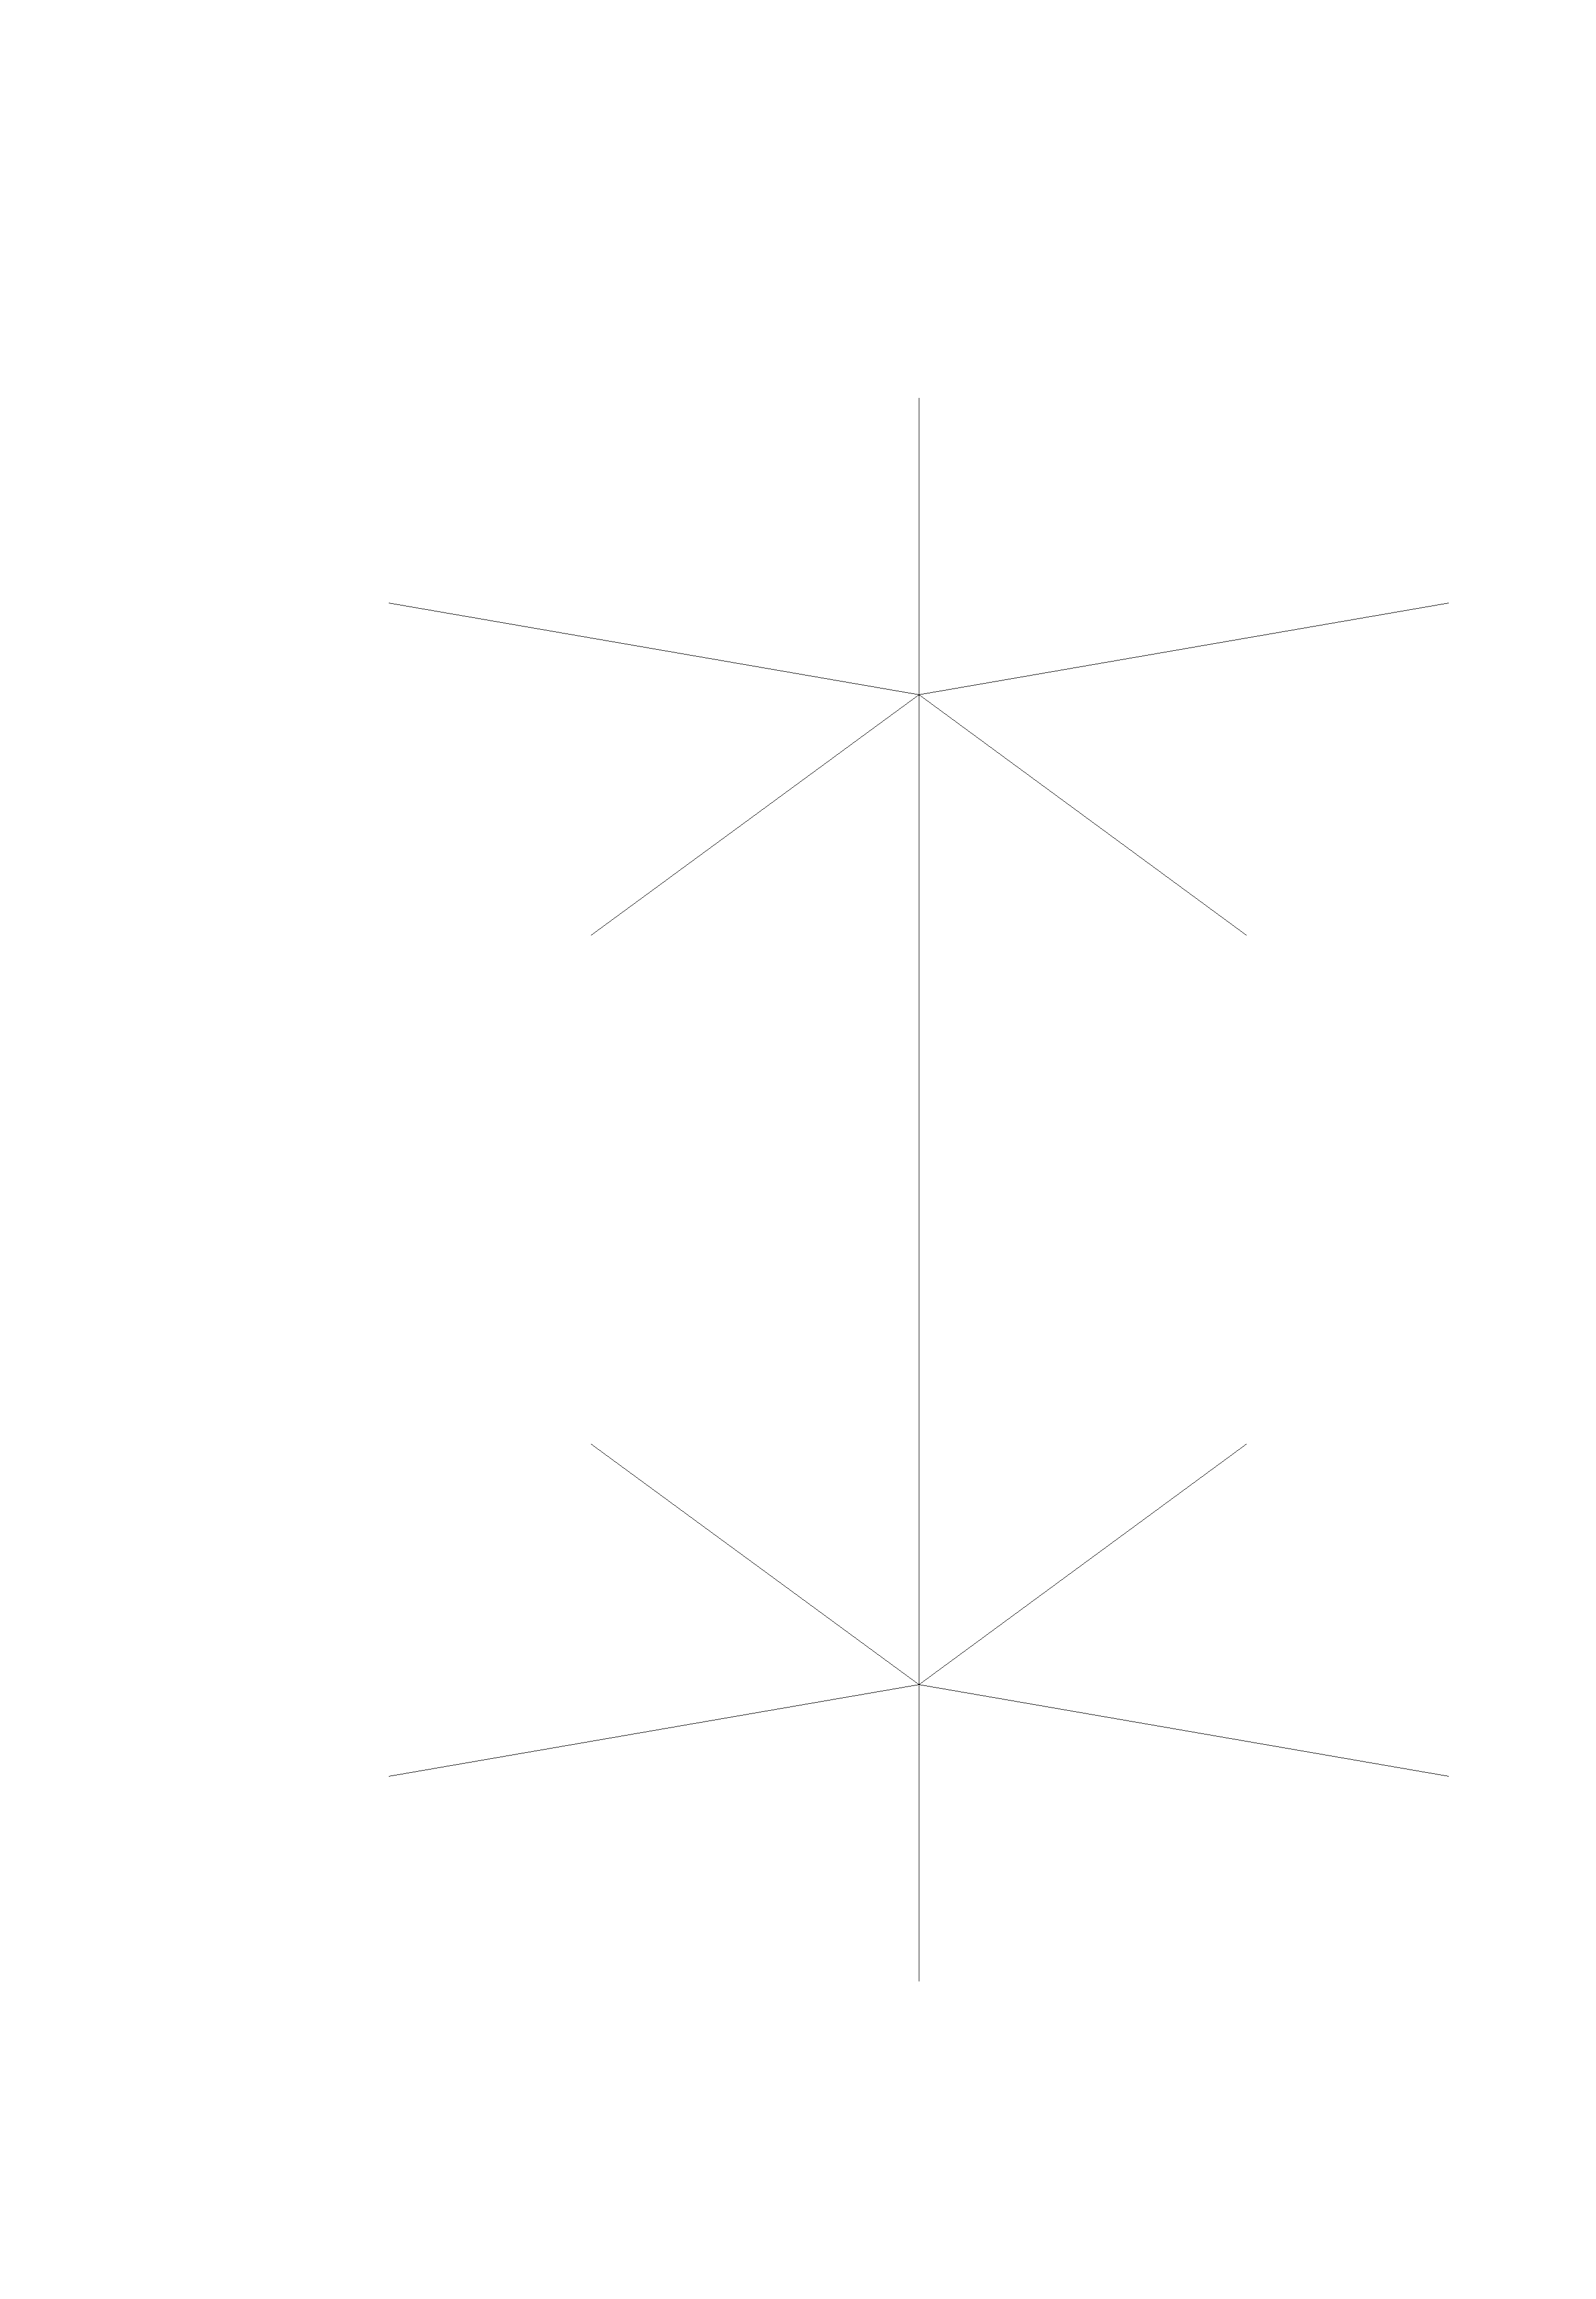
\epsfig{file = ../figures/FigNetworks-Star.eps, height=1.7cm,
      width=4cm, clip=, bbllx=120, bblly=260, bburx=530,
      bbury=570}   \end{tabular}
  & 4
  & $\left( \begin{array}{cccc} 0&1&0&0\\ 1&0&1&0\\0&1&0&1\\0&0&1&0\\
    \end{array} \right)$
  & 0 \\
  \hline \begin{tabular}{p{2cm}} Clusters (affiliation networks)
  \end{tabular}
  
  & \begin{tabular}{c} 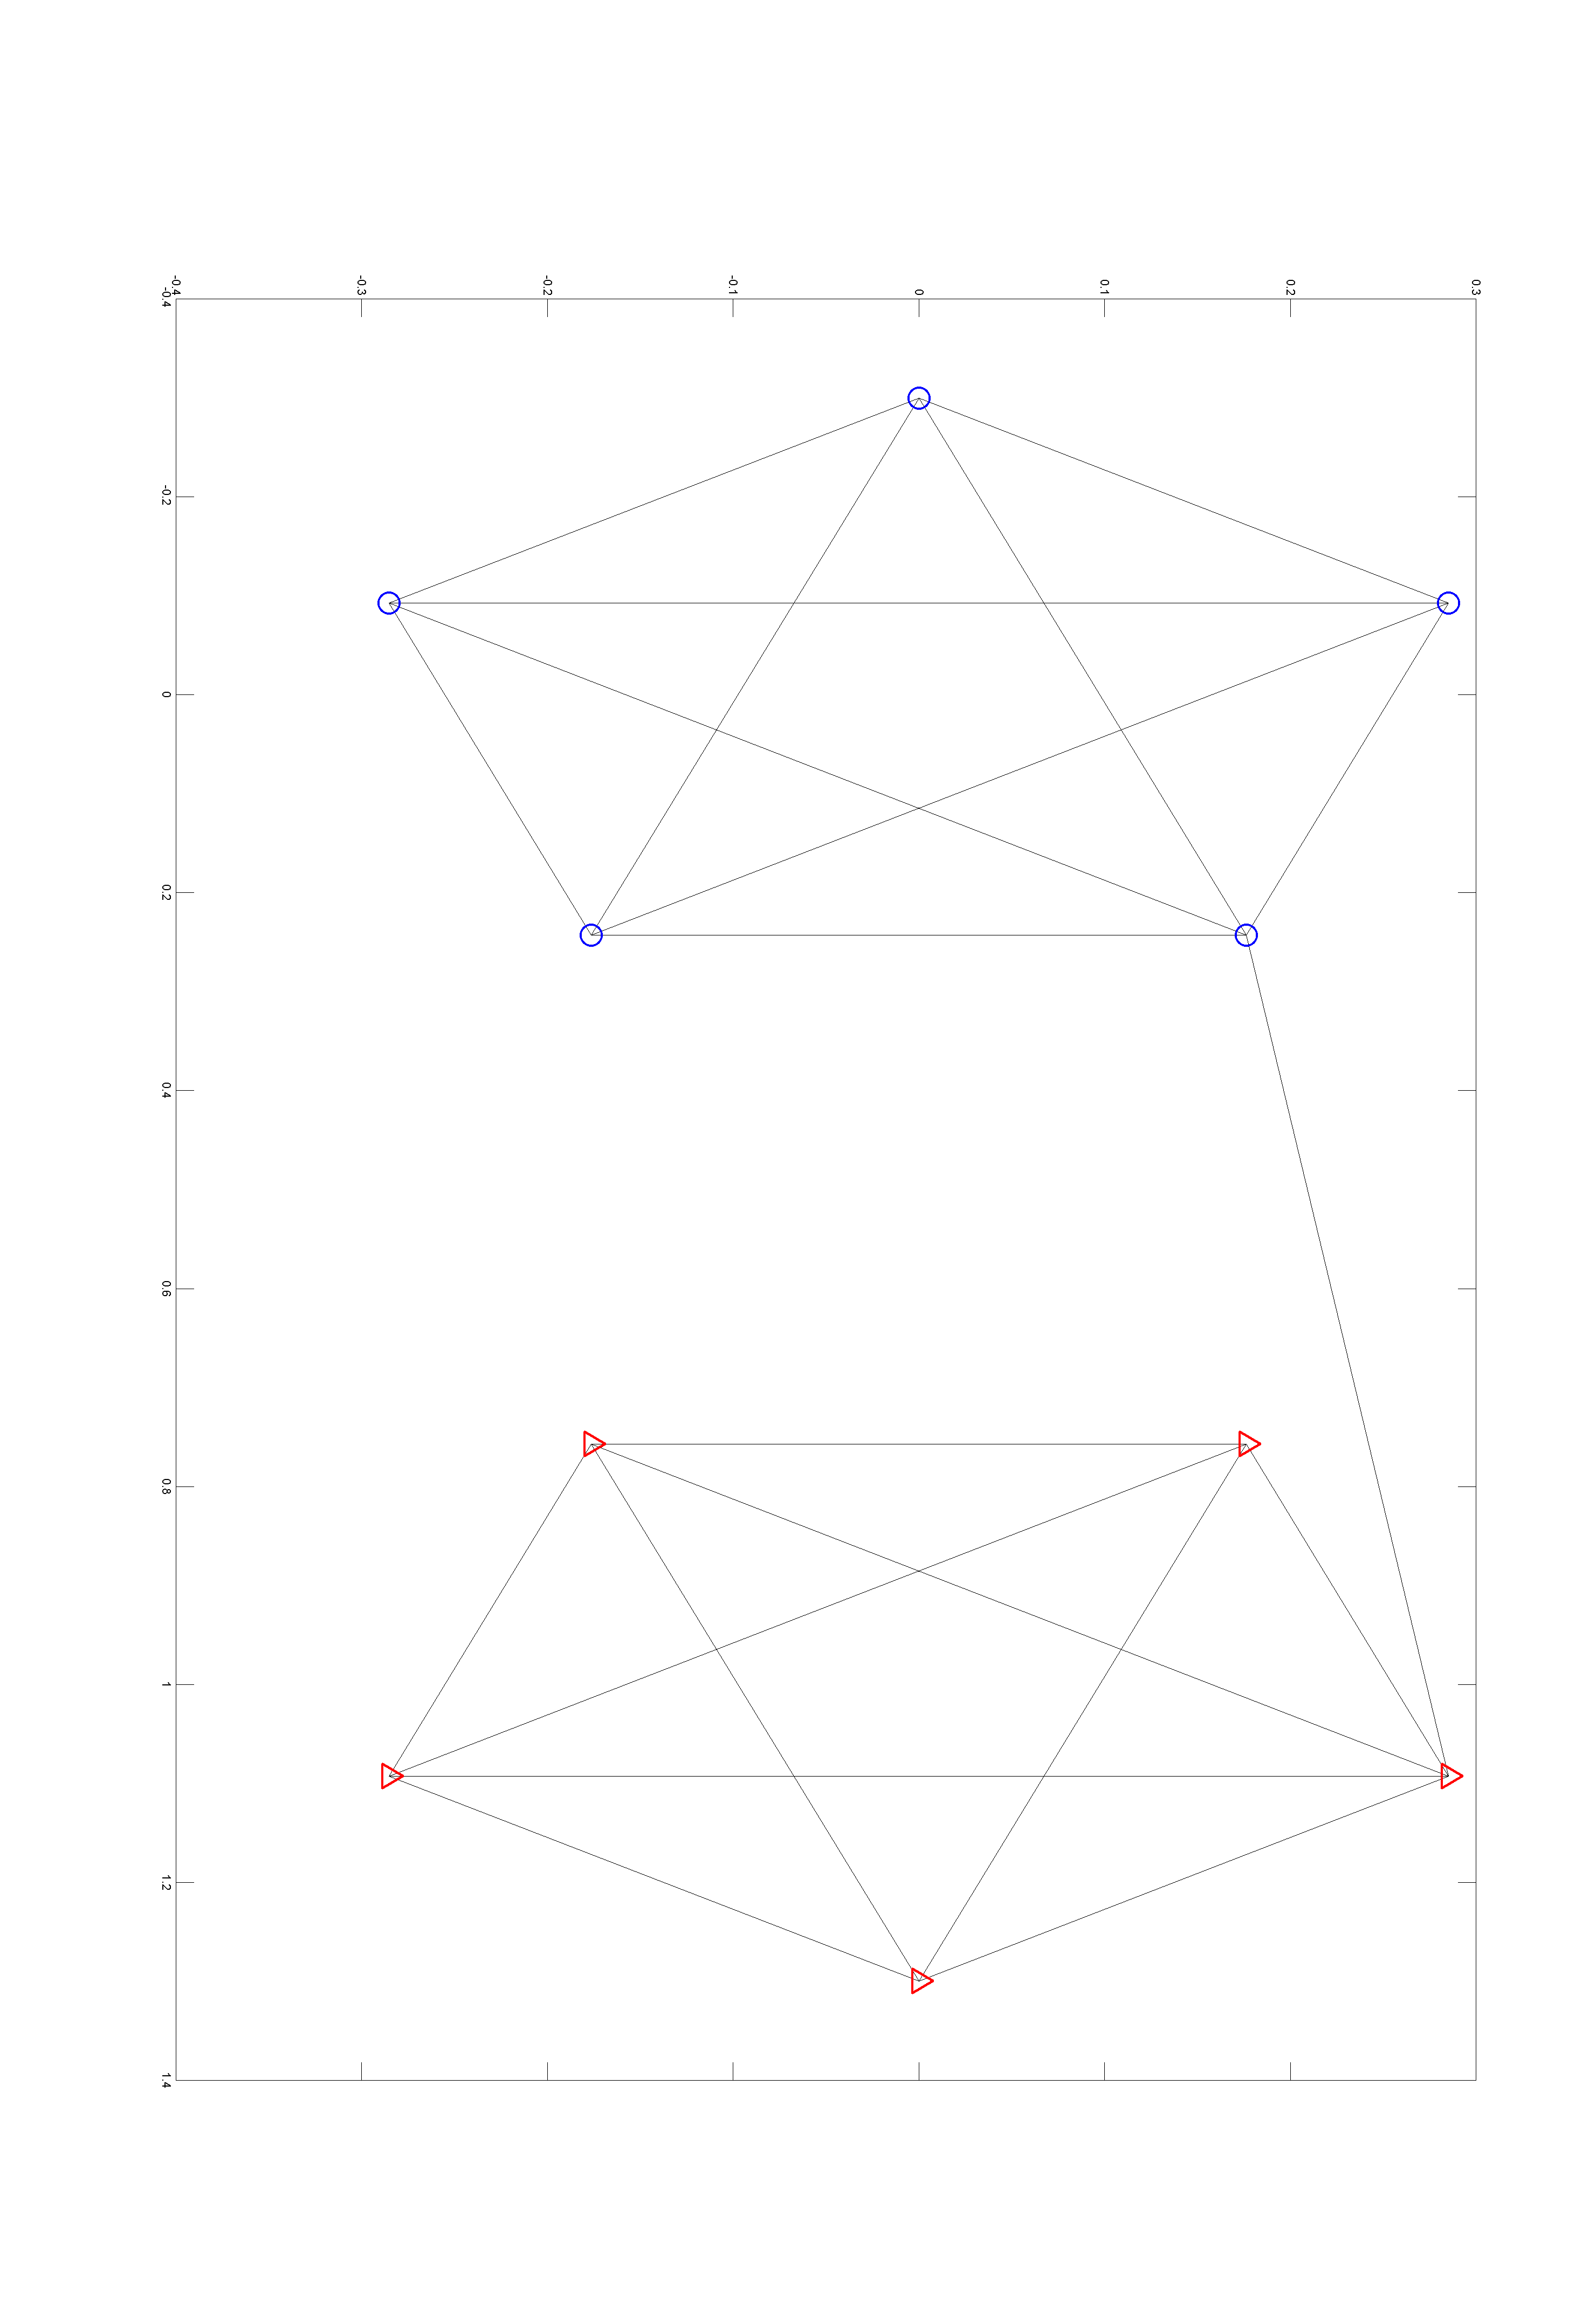
\epsfig{file = ../figures/FigNetworks-Clusters.eps,
      height=1.8cm, width=4cm, clip=, bbllx=120, bblly=260, bburx=530,
      bbury=570}  \end{tabular}
  & 2
  & $\left(\begin{array}{cc} 1&\varepsilon\\ \varepsilon&1\\
    \end{array} \right)$ &
  $\displaystyle{\frac{1+3\varepsilon^2}{(1+\varepsilon)^2}}$ \\ 
\end{tabular} \\
\\
\paragraph{Scale free network model }
(Barabasi \& Albert, 99) can also be expressed in terms of ERMG.

%%%%%%%%%%%%%%%%%%%%%%%%%%%%%%%%%%%%%%%%%%%%%%%%%%%%%%%%%%%%%%%%%%%%%
\newpage
\subsection{Some properties of the ERMG model}
%%%%%%%%%%%%%%%%%%%%%%%%%%%%%%%%%%%%%%%%%%%%%%%%%%%%%%%%%%%%%%%%%%%%%

\bigskip
\paragraph{Conditional distribution of the degrees:}
$
K_i \;|\; \{i \in q \} \sim \Bcal(n-1, \pibar_q) \approx
\Pcal(\lambda_q)
$
where $ \pibar_q = \sum_{\ell} \alpha_{\ell} \pi_{q\ell}$,
$\lambda_q = (n-1) \pibar_q$.

\bigskip
\paragraph{Marginal distribution = mixture:}
$$ K_i \sim \sum_q \alpha_q \Bcal(n-1, \pibar_q) \approx \sum_q \alpha_q
\Pcal(\lambda_q).  $$

\bigskip
\paragraph{Between-group connectivity.}
$A_{q\ell}$ denotes the connectivity between groups $q$ and $\ell$:
$$
A_{q\ell} = \sum_{i<j} Z_{iq} Z_{j\ell} X_{ij}, 
\qquad
\Esp (A_{q\ell})  = n(n-1) \alpha_q \alpha_{\ell} \pi_{q\ell} \left/ 2
  \right..
$$

\bigskip
\paragraph{Clustering coefficient:}  
$$
c = \Pr\{\nabla \;|\; \Vsf\} = \Pr\{\nabla\} /
\Pr\{\Vsf\} = \frac{\sum_{q, \ell, m} \alpha_q \alpha_{\ell} \alpha_m
  \pi_{q\ell} \pi_{qm} \pi_{\ell m}}{\sum_{q, \ell, m} \alpha_q
  \alpha_{\ell} \alpha_m \pi_{q\ell} \pi_{qm}}.
$$


%%%%%%%%%%%%%%%%%%%%%%%%%%%%%%%%%%%%%%%%%%%%%%%%%%%%%%%%%%%%%%%%%%%%%
\newpage
\chapter{Maximum likelihood estimation via E-M}
%%%%%%%%%%%%%%%%%%%%%%%%%%%%%%%%%%%%%%%%%%%%%%%%%%%%%%%%%%%%%%%%%%%%%

We denote $\Xcal = \{X_{ij}\}_{i, j = 1..n}$, $\Zcal=
\{Z_{iq}\}_{i=1..n, q=1..Q}$.

%%%%%%%%%%%%%%%%%%%%%%%%%%%%%%%%%%%%%%%%%%%%%%%%%%%%%%%%%%%%%%%%%%%%%
\subsection{Likelihood}
%%%%%%%%%%%%%%%%%%%%%%%%%%%%%%%%%%%%%%%%%%%%%%%%%%%%%%%%%%%%%%%%%%%%%

The conditional expectation of the complete-data log-likelihood is
\begin{eqnarray*}
  \Qcal(\Xcal) &=& \Esp \left\{ \Lcal(\Xcal,\Zcal)|\Xcal \right\}  \\
  \\
  &=&  \sum_i \sum_q \tau_{iq} \log \alpha_q
  + \sum_i \sum_q \sum_{j > i} \sum_{\ell} \theta_{ijq\ell} \log
  b(X_{ij}; \pi_{q\ell}),
\end{eqnarray*}
where $\tau_{iq}$ and $\theta_{ijq\ell}$ are {\it posterior}
probabilities
$$
\tau_{iq} = \Pr\{Z_{iq} = 1 \;|\; \Xcal\}, \qquad
\theta_{ijq\ell} = \Pr\{Z_{iq} Z_{j\ell} = 1 \;|\; \Xcal\}
$$
% \begin{eqnarray*}
%   \tau_{iq} & = & \Pr\{Z_{iq} = 1 \;|\; \Xcal\} = \Esp(Z_{iq} \;|\;
%   \Xcal), \\
%   \\
%   \theta_{ijq\ell} & = & \Pr\{Z_{iq} Z_{j\ell} = 1 \;|\; \Xcal\} =
%   \Esp(Z_{iq} Z_{j\ell} \;|\; \Xcal). 
% \end{eqnarray*}
Evaluating these probabilities is not straightforward because the
$\{Z_{iq}\}$ are all dependent conditionally on $\Xcal$.

%%%%%%%%%%%%%%%%%%%%%%%%%%%%%%%%%%%%%%%%%%%%%%%%%%%%%%%%%%%%%%%%%%%%%
\newpage
\paragraph{E step: Mean field approximation.}
We approximate the conditional joint distribution of the $\{Z_{iq}\}$:
\begin{eqnarray*}
  \Pr\{\Zcal \;|\; \Xcal\} & \simeq & \prod_i \Pr\{\Zcal_i \;|\; \Xcal,
  \Zcal^i\} \\
  \quad \mbox{where} \quad
  \Pr\{Z_{iq} = 1 \;|\; \Xcal, \Zcal^i\} & \propto & \alpha_q \prod_{m}
  b(C_{im}; N^i_{m} , \pi_{qm})
\end{eqnarray*}
\begin{itemize}
\item The elements of $\Zcal^i$ are estimated by their conditional
  expectation: $ \widehat{Z}_{j\ell} = \tau_{j\ell}$.
\item The posterior probabilities $\tau_{iq}$ must therefore satisfy 
  $$
  \widehat{\tau}_{iq} = \Pr\{Z_{iq} = 1 \;|\; \Xcal,
  \widehat{\Zcal}^i\} 
  $$
  which is actually a fix point type relation.  The
  $\widehat{\tau}_{iq}$ are obtained by iterating it.
\end{itemize}

\paragraph{M step.}
Maximizing $\Qcal(\Xcal)$ subject to $\sum_q \alpha_q = 1$ gives
$$
\widehat{\alpha}_q = \sum_i \widehat{\tau}_{iq} / n, \qquad
\widehat{\pi}_{q\ell} = \sum_i \sum_j \widehat{\theta}_{ijq\ell}
X_{ij} \left/ \sum_i \sum_j \widehat{\theta}_{ijq\ell} \right..
$$

%%%%%%%%%%%%%%%%%%%%%%%%%%%%%%%%%%%%%%%%%%%%%%%%%%%%%%%%%%%%%%%%%%%%%
\newpage
\subsection{Choice of the number of groups}
%%%%%%%%%%%%%%%%%%%%%%%%%%%%%%%%%%%%%%%%%%%%%%%%%%%%%%%%%%%%%%%%%%%%%

We propose a heuristic penalized likelihood criterion inspired from
BIC.

Since $\Qcal(\Xcal)$ is the sum of
$$
\begin{tabular}{p{11cm}p{13cm}}
  $\displaystyle{\sum_i \sum_q \tau_{iq} \log \alpha_q}$ & 
  which deals with $(Q-1)$ independent proportions $\alpha_q$s and
  involves $n$ terms, 
  \\ 
  \\
  $\displaystyle{\sum_i \sum_q \sum_{j > i} \sum_{\ell} \theta_{ijq\ell} \log
    b(X_{ij}; \pi_{q\ell})}$ 
  & which deals with $Q(Q+1)/2$ probabilities $\pi_{q\ell}$s and
  involves $n(n-1)/2$ terms,
\end{tabular}
$$
we propose the following heuristic criterion:
$$
  - 2\Qcal(\Xcal) + (Q-1) \log n + Q(Q+1)/2 \log[n(n-1)/2].
$$

%%%%%%%%%%%%%%%%%%%%%%%%%%%%%%%%%%%%%%%%%%%%%%%%%%%%%%%%%%%%%%%%%%%%%
\newpage
\chapter{Application to {\it E. coli} reaction network}
%%%%%%%%%%%%%%%%%%%%%%%%%%%%%%%%%%%%%%%%%%%%%%%%%%%%%%%%%%%%%%%%%%%%%

Fit of the ERMG model to a graph with $n=605$ vertices and $1\;782$
edges.

\paragraph{`Optimal' number of groups:} $Q = 21$.

\paragraph{Group proportions.} $\widehat{\alpha}_q$ (\%).
$$
\epsfig{file = ../figures/Ecoli-Complet-ERMG-Ward-Q21_param.eps, height=6cm,
  width=12cm, clip=, bbllx=75, bblly=570, bburx=530, bbury=770}  
$$
Many small groups actually correspond to cliques or pseudo-cliques.

% The first three groups are actually three cliques of size 14, 18 and 21.

% No connection exists between the first two cliques. 

% Vertices from group 3 have rather frequent connections with group 4.

% The clique structure strongly increases the mean degree $\lambda_q$ of
% its elements.

%%%%%%%%%%%%%%%%%%%%%%%%%%%%%%%%%%%%%%%%%%%%%%%%%%%%%%%%%%%%%%%%%%%%%
\newpage
\hspace{-2cm}
\begin{tabular}{cc}
  \begin{tabular}{p{11cm}}
    \paragraph{Dot-plot representation of the graph.} \\ \\
    Dot present means 
    $$X_{ij} = 1$$
    The vertices are re-ordered according to their 'mean group
    number':
    $$
    \widehat{q}_i = \sum_q q \; \widehat{\tau}_{iq} 
    $$
  \end{tabular}
  &
  \begin{tabular}{c}
    \epsfig{file = ../figures/Ecoli-Complet-ERMG-Ward-Q21_class.eps,
      height=13cm, width=13cm, clip=,bbllx=70, bblly=440, bburx=540,
      bbury=770}   
  \end{tabular} 
  \vspace{-1cm}
  \\
  \begin{tabular}{p{11cm}}
    \paragraph{Posterior probabilities $\widehat{\tau}_{iq}$.}  \\ \\ \\
  \end{tabular}
  & 
  \begin{tabular}{c}
    \epsfig{file = ../figures/Ecoli-Complet-ERMG-Ward-Q21_class.eps,
    width=13cm, clip=, bbllx=70, bblly=265, bburx=540, bbury=420}  
  \end{tabular}
\end{tabular}
%$$

%%%%%%%%%%%%%%%%%%%%%%%%%%%%%%%%%%%%%%%%%%%%%%%%%%%%%%%%%%%%%%%%%%%%%
\newpage
\hspace{-2cm}
\begin{tabular}{cc}
  \begin{tabular}{p{9cm}}
    \paragraph{Zoom (bottom left).} \\ 
    \\
    Submatrix of $\pi$:
    $$
    \begin{tabular}{c|cccc}
      $q, \ell$ & 1 & 9 & 10 & 16 \\
      \hline 
      1 & \paragraph{\bf 1.0} \\ 
      9 & \paragraph{\sl .11} & .65 \\ 
      10 & \paragraph{\sl .43} & & .67  \\ 
      16 & \paragraph{\bf 1.0} & \paragraph{\sl .01} & & \paragraph{\bf 1.0} \\ 
    \end{tabular}
    $$
    \\ \\ 
  \end{tabular}
  &
  \begin{tabular}{l}
    \hspace{1.3cm}
    \epsfig{file = ../figures/Ecoli-Complet-ERMG-Ward-Q21_class.eps,
      height=12cm, width=12cm, clip=,bbllx=90, bblly=485, bburx=277,
      bbury=605.5}   
  \end{tabular}  
  \vspace{-2cm}
  \\ \\ \\
  \begin{tabular}{p{9cm}}
    \paragraph{Vertices degree $K_i$.}  \\ \\ 
    Mean degree in the last group:\\ 
    $\overline{K}_{21} = 2.6$ \\ \\ \\
  \end{tabular}
  & 
  \begin{tabular}{l}
    \epsfig{file = ../figures/Ecoli-Complet-ERMG-Ward-Q21_class.eps,
    width=13.4cm, height=6cm, clip=, bbllx=70, bblly=105, bburx=277,
    bbury=245}   
  \end{tabular}
\end{tabular}

%%%%%%%%%%%%%%%%%%%%%%%%%%%%%%%%%%%%%%%%%%%%%%%%%%%%%%%%%%%%%%%%%%%%%
\newpage
\hspace{-2cm}
\begin{tabular}{ll}
  \begin{tabular}{p{11cm}}
    \paragraph{Between group connectivity.} \\
    Observed vs predicted: quite good \\ \\ 
    but the 'observed' $A_{q\ell}$ are not observed but estimated with the MAP
    rule:
    $$
    {\widehat{A}_{q\ell} = \sum_{i<j} \widehat{Z}_{iq}
      \widehat{Z}_{j\ell} X_{ij}}
    $$
    so the observed good fit is optimistic. \\ \\ \\
  \end{tabular}
  & 
  \begin{tabular}{c}
    \epsfig{file =
      ../figures/Ecoli-Complet-ERMG-Ward-Q21_param.eps, height=10cm,
      width=10cm, clip=, bbllx=70, bblly=300, bburx=530, bbury=530}   
  \end{tabular}
\end{tabular}


\paragraph{Clustering coefficient.}
$$
\begin{tabular}{cccc}
  Empirical & ERMG ($Q = 6$) & ERMG ($Q = 21$) & ER ($Q = 1$)\\
  \hline
  0.626 & 0.436 & 0.544 & 0.0098
\end{tabular}
$$

%%%%%%%%%%%%%%%%%%%%%%%%%%%%%%%%%%%%%%%%%%%%%%%%%%%%%%%%%%%%%%%%%%%%%%%%
\newpage
%$$
\vspace{-2cm}
\hspace{-2cm}
\begin{tabular}{cc}
  \begin{tabular}{l}
    \paragraph{Reaction graph.} \\ \\ 
    Groupe number \\
    (group size) \\ \\ \\ \\ \\ \\ \\ \\ \\ \\ \\ \\ \\ \\ \\ 
  \end{tabular}
  &
  \begin{tabular}{l}
    \epsfig{file = ../figures/Ecoli-Complet-ERMG-Ward-Q21_graph.eps, height=18cm,
      width=18cm, clip=, bbllx=130, bblly=170, bburx=500, bbury=700} 
  \end{tabular}
\end{tabular}
%$$

%%%%%%%%%%%%%%%%%%%%%%%%%%%%%%%%%%%%%%%%%%%%%%%%%%%%%%%%%%%%%%%%%%%%%%%%
\newpage
\chapter{Conclusions}

\paragraph{Past.} 
\begin{itemize}
\item \vspace{-0.5cm} The ERMG model is a flexible generalization of
  the ER model and a promising alternative to the scale-free 'model'.
\item \vspace{-0.5cm} It seems to fit well several real-world networks
  %(Airport network, Enzyme network in bacteria, etc.).
\item \vspace{-0.5cm} It is properly defined, so its properties can be
  properly studied.
\end{itemize}

\paragraph{Future.}
\begin{itemize}
\item \vspace{-0.5cm} Study the probabilistic properties of the ERMG
  model (diameter, probability for a subgraph to be connected, etc).
\item \vspace{-0.5cm} Derive a relevant criterion to select the number
  of groups.
\item \vspace{-0.5cm} Extension to valued graphs: $X_{ij}$ not only
  0/1, but some measure of the connection intensity.
\end{itemize}

% %%%%%%%%%%%%%%%%%%%%%%%%%%%%%%%%%%%%%%%%%%%%%%%%%%%%%%%%%%%%%%%%%%%%%%%%
% \newpage

% \paragraph{Estimated connection probabilities $\pi_{q\ell}$.} (\%)\\
% %$$
% ${\footnotesize
%   \hspace{-2.5cm}
%   \begin{array}{c|ccccccccccccccccccccc}
% & 1 & 2 & 3 & 4 & 5 & 6 & 7 & 8 & 9 & 10 & 11 & 12 & 13 & 14 & 15 & 16 & 17 & 18 & 19 & 20 & 21 \\ 
% \hline 
% 1 & 100 & & & & & & & & & & & & & & & & & & & &  \\ 
% 2 & & 100 & & & & & & & & & & & & & & & & & & &  \\ 
% 3 & & & 100 & & & & & & & & & & & & & & & & & &  \\ 
% 4 & & & & 71 & & & & & & & & & & & & & & & & &  \\ 
% 5 & & & & & 100 & & & & & & & & & & & & & & & &  \\ 
% 6 & & & & & 28 & 100 & & & & & & & & & & & & & & &  \\ 
% 7 & 64 & & & & & & 58 & & & & & & & & & & & & & &  \\ 
% 8 & & & & & & & & 63 & & & & & & & & & & & & &  \\ 
% 9 & 11 & & & & & & 10 & & 65 & & & & & & & & & & & &  \\ 
% 10 & 43 & & & & 1 & & 4 & & & 67 & & & & & & & & & & &  \\ 
% 11 & & & & & & & & & & & 62 & & & & & & & & & &  \\ 
% 12 & & & 4 & & & & 7 & 5 & & & & 28 & & & & & & & & &  \\ 
% 13 & 2 & & 7 & & & & 5 & & & 1 & & 5 & 100 & & & & & & & &  \\ 
% 14 & & & & & & 6 & & & & & 7 & & & 25 & & & & & & &  \\ 
% 15 & & & 1 & & & & & & & & & & & & 40 & & & & & &  \\ 
% 16 & 100 & & & & 18 & & 5 & & 1 & & & 5 & 1 & & & 100 & & & & &  \\ 
% 17 & & & & & & & & & 2 & & 4 & & & & & & 100 & & & &  \\ 
% 18 & & & 1 & & & & & 3 & 2 & & & & & & & & & 21 & & &  \\ 
% 19 & & & & & 16 & & & & & & & & & & & & 0 & & 19 & &  \\ 
% 20 & & & & & & & & & & & & & & & 0 & & 6 & & 0 & 11 &  \\ 
% 21 & & 0 & 0 & 0 & 0 & 0 & 0 & 0 & 0 & 0 & 0 & 0 & 0 & 0 & 0 & 0 & 0 & 0 & 0 & 0 & 1  \\ 
%   \end{array}
% }$
% %$$


%%%%%%%%%%%%%%%%%%%%%%%%%%%%%%%%%%%%%%%%%%%%%%%%%%%%%%%%%%%%%%%%%%%%%%%%
%%%%%%%%%%%%%%%%%%%%%%%%%%%%%%%%%%%%%%%%%%%%%%%%%%%%%%%%%%%%%%%%%%%%%%%%
%%%%%%%%%%%%%%%%%%%%%%%%%%%%%%%%%%%%%%%%%%%%%%%%%%%%%%%%%%%%%%%%%%%%%%%%
%%%%%%%%%%%%%%%%%%%%%%%%%%%%%%%%%%%%%%%%%%%%%%%%%%%%%%%%%%%%%%%%%%%%%%%%
\end{document}
%%%%%%%%%%%%%%%%%%%%%%%%%%%%%%%%%%%%%%%%%%%%%%%%%%%%%%%%%%%%%%%%%%%%%%%%
%%%%%%%%%%%%%%%%%%%%%%%%%%%%%%%%%%%%%%%%%%%%%%%%%%%%%%%%%%%%%%%%%%%%%%%%
%%%%%%%%%%%%%%%%%%%%%%%%%%%%%%%%%%%%%%%%%%%%%%%%%%%%%%%%%%%%%%%%%%%%%%%%
%%%%%%%%%%%%%%%%%%%%%%%%%%%%%%%%%%%%%%%%%%%%%%%%%%%%%%%%%%%%%%%%%%%%%%%%

